\documentclass[10pt,pdf,hyperref={unicode}]{beamer}


% \documentclass[aspectratio=43]{beamer}
% \documentclass[aspectratio=1610]{beamer}
% \documentclass[aspectratio=169]{beamer}

\usepackage{multicol}
\usepackage{lmodern}
\usepackage{lipsum}
\usepackage{marvosym}
\usepackage{amssymb}

% подключаем кириллицу 
%\usepackage[T1,T2A]{fontenc}
\usepackage[lutf8]{luainputenc}
\usepackage[english,russian]{babel}

% отключить клавиши навигации
\setbeamertemplate{navigation symbols}{}

% тема оформления
\usetheme{CambridgeUS}
% цветовая схема
\usecolortheme{crane}

\usepackage{fontspec}
        \defaultfontfeatures{Ligatures={TeX}}
        \setmainfont{Ubuntu}
        \setsansfont{Ubuntu}
        \setmonofont{Ubuntu Mono}
    \usepackage[english,russian]{babel}

\date{}

\title[]{...ers,Developers,Developers,Developers,Dev...}   
%\subtitle{Use beamer everywhere you are}
\author[]{Кирпиченков Денис} 
\institute[]{Naumen}
%\date{\today} 
% \logo{\includegraphics[height=5mm]{images/logo.png}\vspace{-7pt}}

\begin{document}

% титульный слайд
\begin{frame}
\titlepage
\end{frame} 

\begin{frame}
\frametitle{История о разработке одного продукта} 

\begin{itemize}
\item Время разработки 10 лет
\item 3 перерождения: Python, Java + JSP, Java + GWT
\item ~1 000 000 строк java-кода, 60 000 строк скриптов
\item Распределенная команда из 20 разработчиков в 3 городах
\end{itemize}

\end{frame}

\begin{frame}
\frametitle{Read,Code,Debug,Test... Repeat} 

\begin{columns}[T]
	\column{0.3\textwidth}
		\center
			Общие алгоритм работы
		\begin{enumerate}

			\item прочитать требования;
			\item реализовать;
			\item показать реализацию;
			\item отдать в тестирование;
			\item goto 1/goto 2.
	
		\end{enumerate}
	\column{0.3\textwidth}
		\center
			Исправление дефектов
		\begin{enumerate}
			\item воспроизвести дефект;
			\item проанализировать причины;
			\item исправить поведение.
		\end{enumerate}
	\column{0.3\textwidth}
		\center
			Улучшение (производительности) продукта
		\begin{enumerate}
			\item проанализировать проблему;
			\item замерить текущие показатели;
			\item исправить;
			\item замерить новые показатели;
			\item goto 3.
		\end{enumerate}
	\end{columns}
\end{frame}

\begin{frame}
\frametitle{Что общего у (почти) всех программистов} 

\center

\includegraphics[height=0.6\textheight]{./multi_fun.png}

\end{frame}

\begin{frame}
\frametitle{void function career() \{ while(1) \{ doCodeALot() \} \} }
\framesubtitle{ обощенный путь разработчика }

\begin{columns}[T]
	\column{0.5\textwidth}

		\begin{itemize}
			\item Стажер
			\item Разработчик
			\item Ведущий разработчик
		\end{itemize}

	\column{0.5\textwidth}

		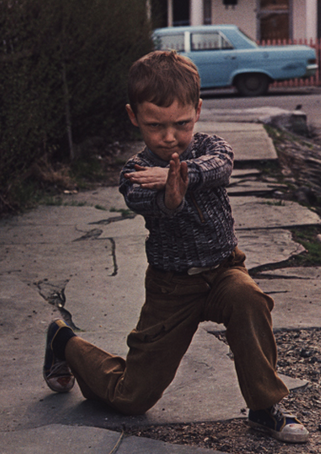
\includegraphics[width=0.5\textwidth]{./intern.png}
		
\includegraphics[width=0.484\textwidth]{./senior.png}

\end{columns}

\end{frame}

\begin{frame}
	\frametitle{``Типы'' программистов }
		\begin{itemize}
			\item Embedded разработка
			\item Enterprise разработка
			\item Mobile разработка
		\end{itemize}		

		\em
			\begin{itemize}
				\item Gamedev
				\item Desktop-приложения
			\end{itemize}		

\end{frame}


\begin{frame}
\frametitle{ Embedded решения }
	\center
		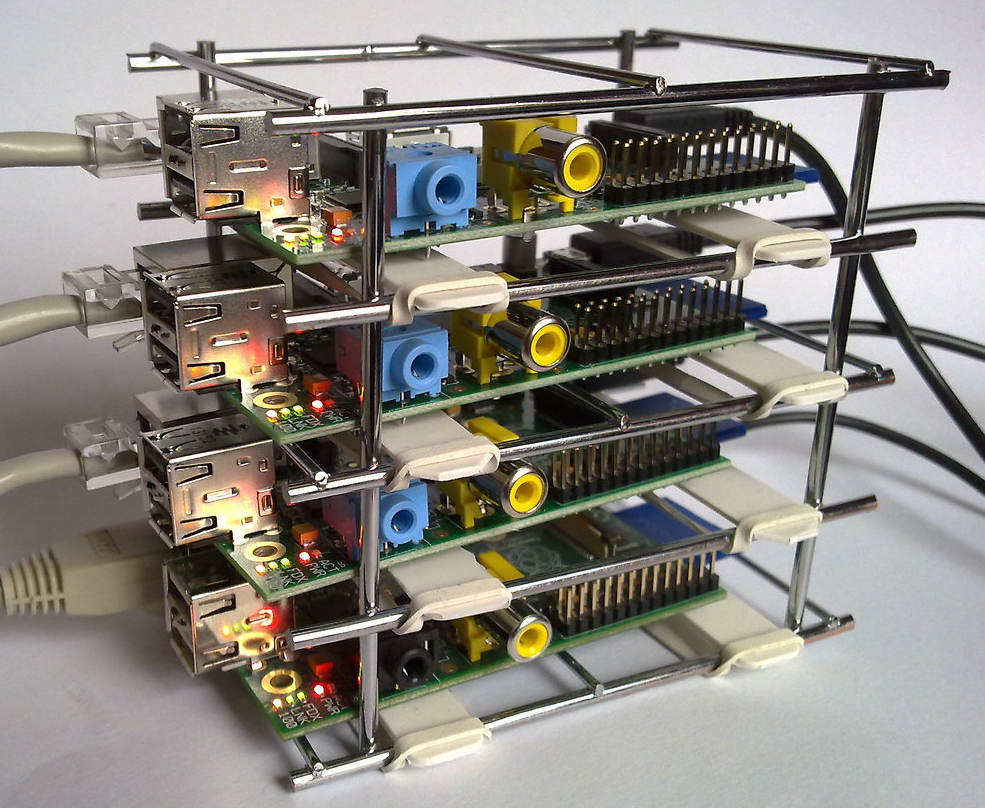
\includegraphics[width=0.7\textwidth]{./rasbery.png}
\end{frame}


\begin{frame}
\frametitle{Enterprise разработка}

\begin{columns}
	\column{0.5\textwidth}
		Версия 1.0
		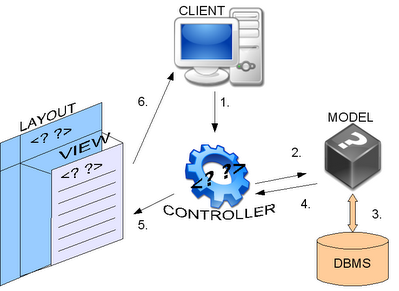
\includegraphics[width=0.8\textwidth]{./ruby.png}
	\column{0.5\textwidth}
		Версия 18.5.2.8
		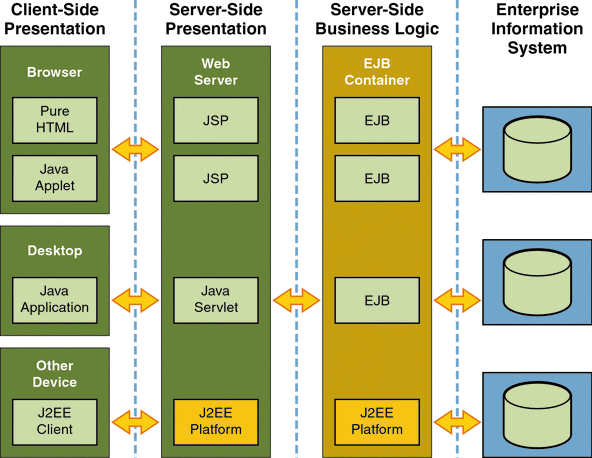
\includegraphics[width=0.8\textwidth]{./enterprise.png}
\end{columns}

\end{frame}

\begin{frame}
\frametitle{ Mobile apps }
	\center
	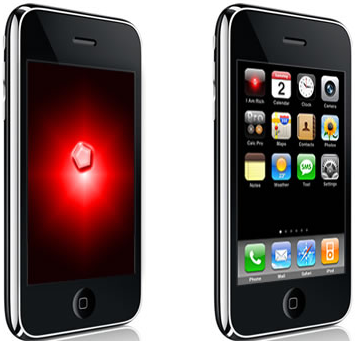
\includegraphics[width=0.4\textwidth]{./imrich.png}
\end{frame}

\begin{frame}
\frametitle{ Hello, world! }
	\center
		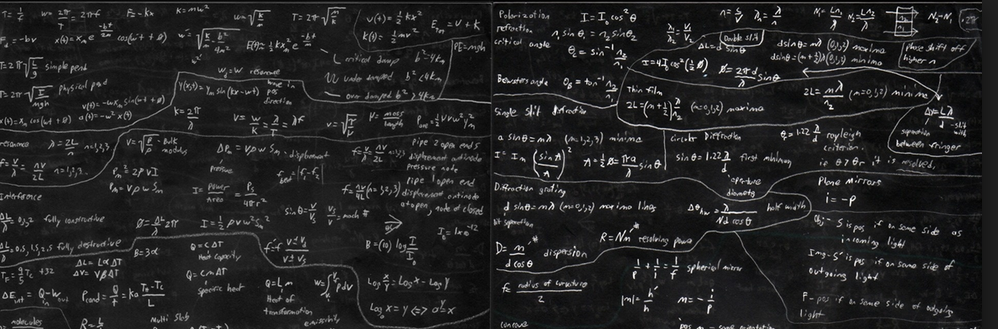
\includegraphics[width=1.0\textwidth]{./haskell.png}		
\end{frame}

\begin{frame}
\frametitle{ Что нужно знать}

\begin{itemize}

	\item Язык программирования
	\item Типы данных
	\item  Особенности аппаратного обеспечения и сети

\end{itemize}

\end{frame}

\begin{frame}
\frametitle{ M x N }

\par
Есть матрица M x N. 

\par
\[
  M=
  \left[ {\begin{array}{ccccc}
   1 & 2 & 3 & 5\\
   3 & 4 & 5 & 7\\
   1 & 2 & 3 & 5\\
   3 & 4 & 5 & 7\\
   1 & 2 & 3 & 5\\
   3 & 4 & 5 & 7\\
  \end{array} } \right]
\]

\par
Цель: обработать все элементы матрицы наиболее эффективным способом.

\par
Как это более эффективно сделать, с точки зрения быстродействия, по колонкам или по строкам матрицы?

\end{frame}

\begin{frame}
\frametitle{ Caveat! }
	\center
		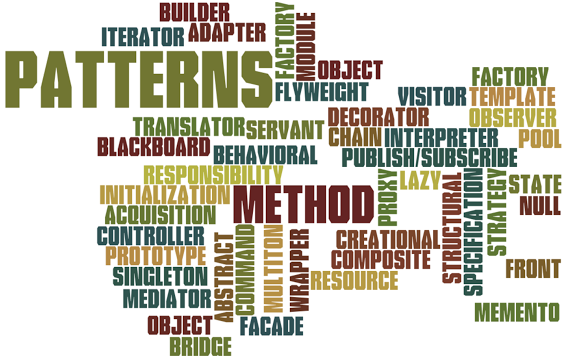
\includegraphics[width=0.8\textwidth]{./antipattern.png}
\end {frame}

\begin{frame}
\frametitle{ Finale }

\center
	
\includegraphics[width=0.8\textwidth]{./run_dos_run.png}

\end{frame}

\begin{frame}
\frametitle{ Finale }

\center
	
\includegraphics[width=0.4\textwidth]{./github.png}

	https://github.com/d0k1/U-R-DEVELOPER

\end{frame}

\end{document}